\section{Spielregeln}
\begin{center}
	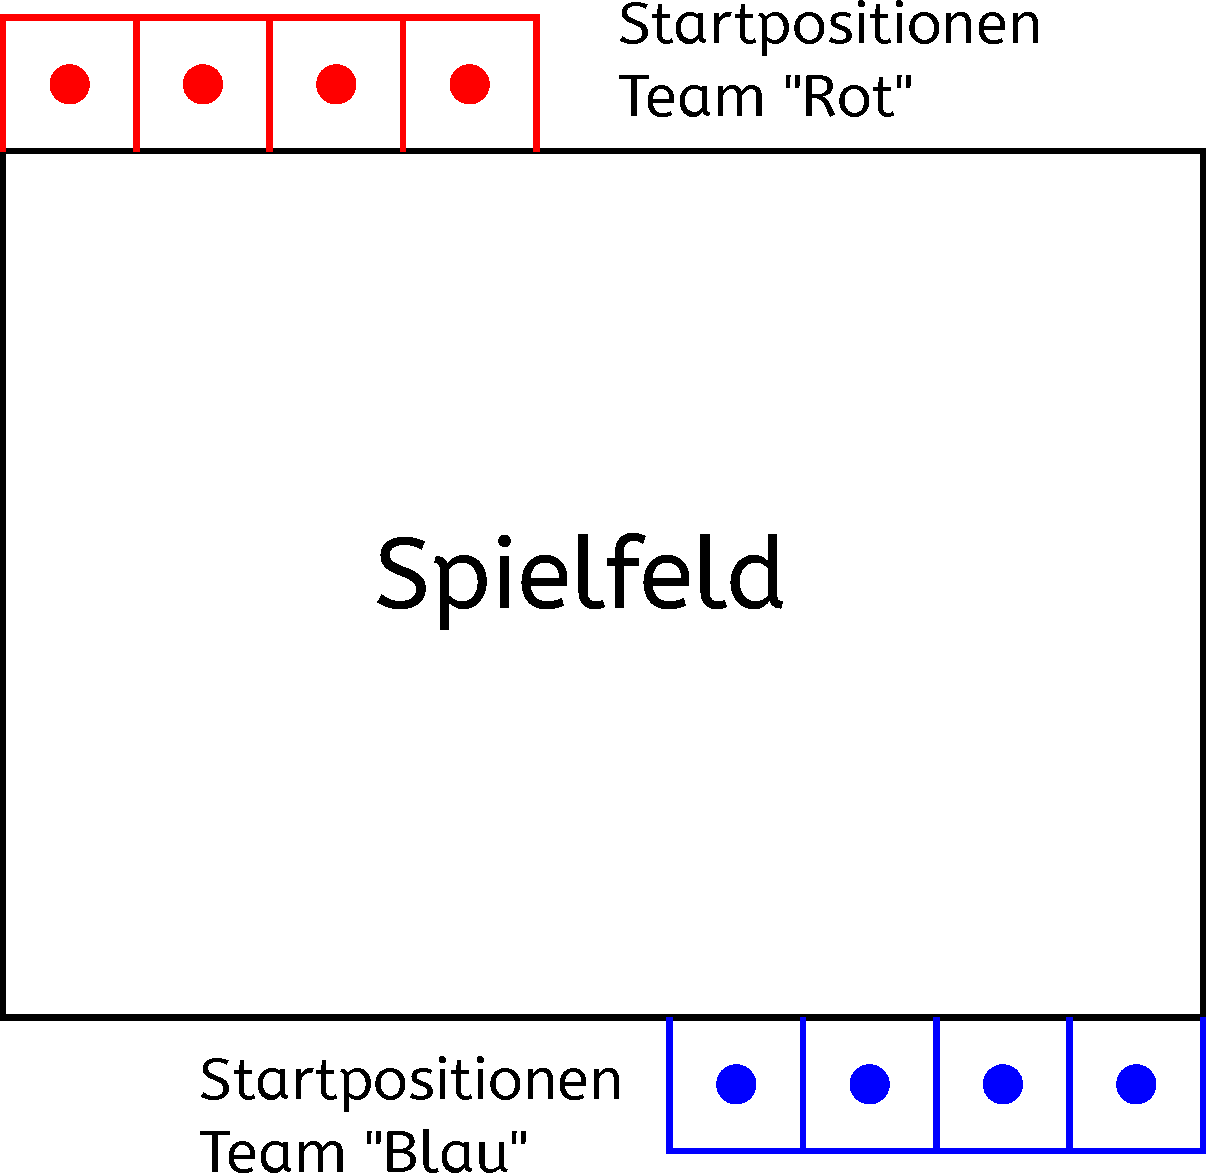
\includegraphics[width=0.5\textwidth]{Bilder/Spielfeld.pdf}
\end{center}
Es werden pro Gruppe 4 Roboter auf dem Spielfeld in extra Positionsfelder platziert.

\begin{enumerate}
	\item "'Start"' an den Server senden
	\item Warten auf Start vom Server
	\item Losfahren
	\item Ab Abstand x vom Gegner, wird die volle Geschwindigkeit freigeschaltet
	\item Meldung ob ein Gegner gefangen wurde, an den Server senden
	\item Server setzt den Gefangenen auf neutral
	\item Gefangener Roboter fährt aus dem Spielfeld
	\item Spiel endet wenn alle Roboter einer Gruppe gefangen wurden bzw. nach 30 Minuten
\end{enumerate}